\chapter{State of the Art\label{cha:chapter2}}
\section{Object Detection Methods}
Two contemporary object detection methods, \textit{Accelerated KAZE} (AKAZE, KAZE meaning wind in Japanese)~\cite{Alcantarilla2012KAZEFeatures, Alcantarilla2013FastSpaces} and \textit{Template Matching} (TM)~\cite{Brunelli2009TemplatePractice}, shall be discussed here briefly.

\subsection{AKAZE}
AKAZE feature matching, introduced in 2013, is a pyramidal object detection algorithm. The Pyramidal approach declines the image ratio with every filtering step. Spanning over several scales, features are detected and described. In contrast to other established algorithms like SIFT which use a linear scale-space for filtering, AKAZE instead uses a nonlinear scale-space with the recently developed numerical model \textit{Fast Explicit Diffusion}. The advantage of the nonlinear scale space is depicted in figure~\ref{skalenraum}: prominent features like edges and corners are preserved. 
\begin{figure}[ht]
	\centering
  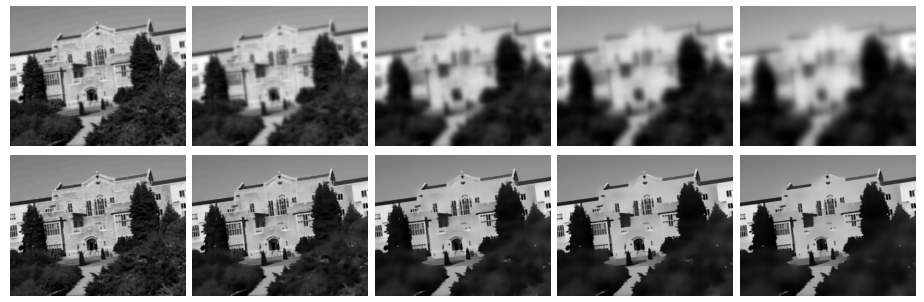
\includegraphics[width=\textwidth]{nonlinearscalespace.png}
	\caption[Gauss filtering]{Top row: Gauss filtering with linear scale space and increasing standard deviation. Bottom Row: Non-linear diffusion scale space.~\cite{Alcantarilla2012KAZEFeatures}}
	\label{skalenraum}
\end{figure}
The outcome of AKAZE is depicted in fig.~\ref{AKAZE}. Matches are shown as dots connected with lines between the two pictures of the same object from another point of view.
\begin{figure}[ht]
	\centering
  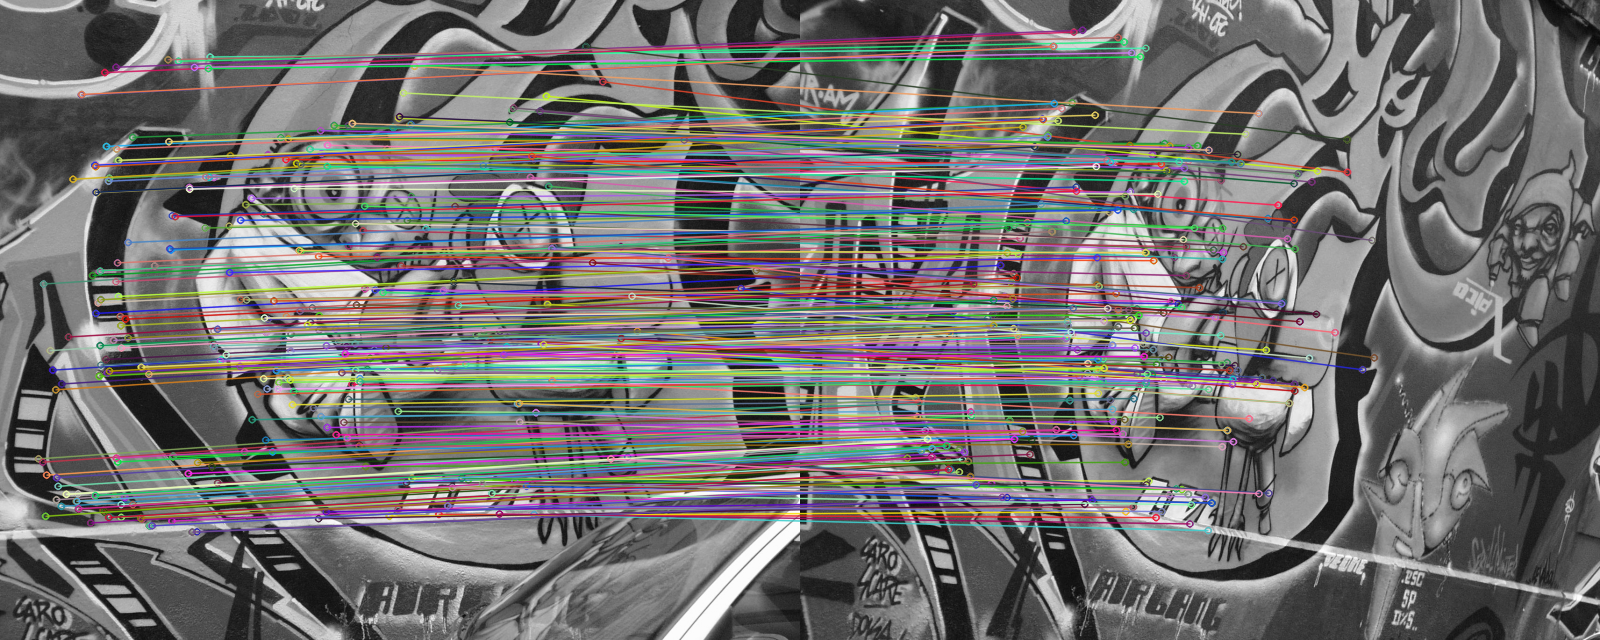
\includegraphics[width=\textwidth]{AKAZE.png}
	\caption[AKAZE Feature Matching]{AKAZE Feature Matching for a graffiti viewed from two different angles. Best viewed in color.~\cite{OpenCV-DocumentationTutorial2018}}
	\label{AKAZE}
\end{figure}

\subsection{Template Matching}
TM was introduced in 2009. Unlike AKAZE, it matches templates instead of features. Fig.~\ref{templatematching} illustrates this process. In the left image, the face of the man is to be found. The template is the little cut-out in the middle. Pixel by pixel, the template is being convoluted with the original image and rated with a metric. The resulting resolution matrix is depicted on the right. Bright areas indicate potential findings. At the brightest point, the template is rightfully suggested.

\begin{figure}[ht]
	\centering
  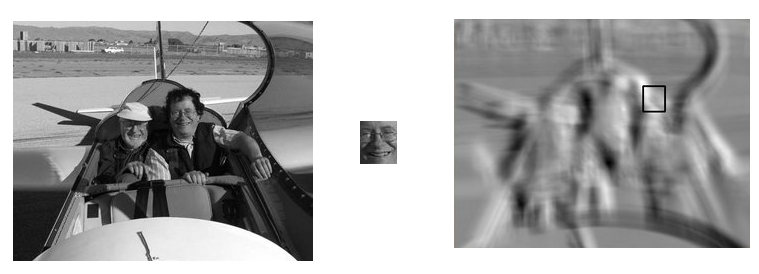
\includegraphics[width=\textwidth]{templatematching.png}
	\caption[Template Matching]{In the picture on the left, the template in the middle is to be found. Depicted on the right is the resolution matrix with potential findings indicated with the bright color and the found area of the template in the original image.~\cite{OpenCV-Documentation2014Template2018}}
	\label{templatematching}
\end{figure}

\subsection{6D Pose Estimation with 3D Training Input}
In recent years, 6D pose estimation gained popularity (see e.g. \cite{Drost2010ModelRecognition}, \cite{Sundermeyer2018ImplicitImages}, \cite{Hinterstoisser2013ModelScenes}). In numerous works, ODMs use a 3D model of an object as training input to generate necessary features or templates. After training, the object can be detected in RGB-D images with the help of the training output. 

In 2018, Hodaň benchmarked 15 ODMs which share this approach.~\cite{Hodan2018BOP:Estimation} He categorized the methods in template-based, feature-based and learning-based. His evaluation showed that feature-based methods currently perform best.

\section{Service-Oriented Architectures}
SOA is a software design paradigm which gained importance towards monolithic approaches. Its main advantages over monolithic approaches are scalability, decoupling of components and simple development, testing and deployment. Service are concise, decoupled components capable of one specific task. The goal is to design services for maximum reusability. Together, either orchestrasted or choreographing, they form an application.

The following subsections focus on how services can be interfaced and deployed.

\subsection {Service Interfaces}
\label{serviceinterfaces}
In this section, potential client-server-based interfaces and underlying protocols shall be discussed. The evaluated interfaces are \textit{Advanced Message Queuing Protocol} (AMQP), \textit{Message Queuing Telemetry Transport} (MQTT), \textit{Representational State Transfer} (REST), \textit{Google Remote Procedure Calls} (gRPC), \textit{Graph Query Language} (GraphQL) and \textit{Open Platform Communication Unified Architecture} (OPC UA).

\subsubsection{AMQP and MQTT}
Both AMQP 0.x and MQTT are broker based protocols specialized for machine-to-machine (M2M) communication. Clients can be sensors, programmable logic controllers, etc.; the server is a broker connecting the clients. A broker is a central instance mediating between parties. Clients can subscribe to various message queues called topics. Telemetry data can then be published and read from these topics handled by the broker. The clients dynamically change between publisher and subscriber. Fig.~\ref{MQTT} illustrates the MQTT architecture.~\cite{Banks2014MQTT2018}

\begin{figure}[ht]
	\centering
  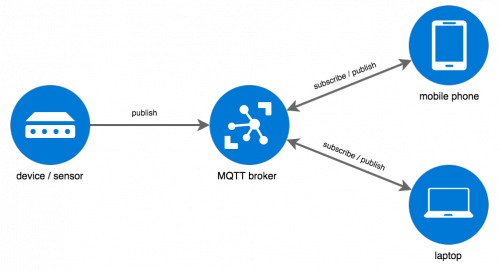
\includegraphics[width=0.9\textwidth]{MQTT.png}
	\caption[MQTT Architecture]{MQTT Architecture with the broker in the middle as a mediator between the clients.~\cite{N.A.Pure-javascript-MQTT-broker.2018}}
	\label{MQTT}
\end{figure}

A commonly used message broker is RabbitMQ which supports AMQP 0.x natively and MQTT via a plugin.~\cite{RabittMQ-Documentation2018Which2018}

AMQP needs to be distinguished between 0.x and 1.0, as the underlying messaging paradigm has been completely revised. While for version 0.x strict publishing/subscription messaging is required, version 1.0 is based on a peer-to-peer connection where a broker is not required, although possible. Due to the more sophisticated version of version 1.0, fewer implementations exist.~\cite{Dizdarevic2018SurveyIntegration}


\subsubsection{REST}
REST is an architectural paradigm describing how distributed systems can communicate with each other. It consists of five mandatory- and one optional restriction/s. If any of the five mandatory restrictions is violated, an architecture cannot be RESTful. The restrictions are client–server architecture, statelessness, cacheability, layered system, uniform interface and code on demand (optional). Roy Fielding developed REST alongside HTTP/1.1 and although it is not dependent on it, HTTP/1.1 is the primarily used protocol to implement REST. Thus, many web pages fulfill these restrictions naturally. REST messages are usually human-readable JSON files. Unlike MQTT or AMQP 0.x, REST does not rely on a broker.~\cite{Fielding2000ArchitecturalArchitectures}

\subsubsection{gRPC}
For many cases in the past, it was hard for maintainers to adhere to all REST principles due to its strict nature. Moreover, REST is usually implemented with HTTP/1.1. In 2015, HTTP/2 was released to address the flaws of its predecessor.~\cite{Sayfan2018REST2018} Among those are the lack of ability of constant data streaming, latency issues, etc. \\ 
gRPC, a remote procedure call technology introduced by Google in 2016, entirely takes advantage of HTTP/2 and thus has some advantages over REST: it allows multiplexing, binary (i.e., quick) data transfer and more. Remote procedure calls let the user call remote methods as if they were local, albeit the remote method can be processed on a different hardware or system. gRPC uses protofiles to describe interface semantics. In protofiles, the user specificies service- and method names as well as message types and input/output values. Out of these protofiles, stubs can be generated which are placeholder classes for gRPC clients and servers. Unlike in most implementations of REST, gRPC does not use textual transport data like JSON but relies on Protobuf, a binary buffer.~\cite{Google-Cloud-Documentation2018Cloud2018} For backwards compatibility towards older clients, there is a gateway available which provides transcoding from HTTP/JSON to gRPC. See figure~\ref{ESP} for the concept behind it.~\cite{N.A.2017Grpc-gateway.2018} 

\begin{figure}[ht]
	\centering
  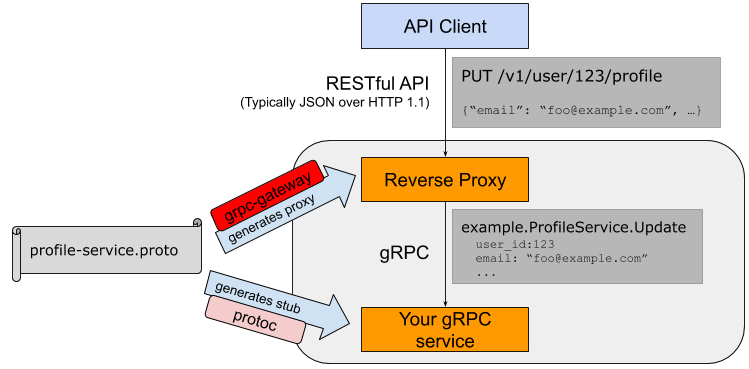
\includegraphics[width=\textwidth]{img/grpc_gateway.png}
	\caption[gRPC gateway concept]{gRPC gateway concept~\cite{N.A.2017Grpc-gateway.2018}}
	\label{ESP}
\end{figure}

The mapping between gRPC and HTTP is desrcibed here with an example directly quoted from Google's API documentation~\cite{Google-API-Documentation2019Http.proto.2019}:\\

\begin{lstlisting}[language=protobuf3,style=protobuf]
     service Messaging {
       rpc GetMessage(GetMessageRequest) returns (Message) {
         option (google.api.http) = {
             get: "/v1/{name=messages/*}"
         };
       }
     }
     message GetMessageRequest {
       string name = 1; // Mapped to URL path.
     }
     message Message {
       string text = 1; // The resource content.
     }
\end{lstlisting}

The option in the protofile enables HTTP REST to gRPC mapping:

    \begin{tabular}{c|c}
        \textbf{HTTP} & \textbf{gRPC} \\ \hline
        GET /v1/messages/123456 & GetMessage(name: "messages/123456")
    \end{tabular}


\subsubsection{GraphQL}
GraphQL is a data query and -manipulation language. It was developed by Facebook and is open-source since 2015. Compared to REST, it has a more flexible and efficient approach. The increase in efficiency over REST is based on faster mobile data access, and more flexibility for the \textit{Application Programming Interface} (API) to let clients access precisely the data they need, i.e., the server modifies the data with respect to the clients' needs instead of providing one rigid resource.~\cite{GraphQL-Documentation2018Basics2018} 

\subsubsection{OPC UA}
OPC UA is a \textit{machine-to-machine} (M2M) protocol specialized in vendor independent communication between heterogeneous machines. On transportation layer, there are three protocols available: binary data over custom \textit{Transmission Control Protocol} (TCP), \textit{Extended Markup Language} (XML) data over \textit{Simple Object Access Protocol} (SOAP), AMQP or MQTT. Due to the higher performance, the former is primarily used nowadays.~\cite{Schleipen2016OPCVariability} Since Publish/Subscribe for OPC UA got introduced on February 6, 2018, in part 14 of the OPC UA specification stack, it is not implemented much yet.

To improve OPC UA's interoperability, \textit{Time Sensitive Networking} has been introduced to the OPC UA environment.~\cite{Wilmes2019ZauberwortKonvergenz} TSN resides on OSI reference model layer 2 as a set of standards (mainly  IEEE 802.1Q,~\cite{IEEE2014IEEENetworks}) to boost networks with low latency and high availability. \textbf{Convergent} networks can be implemented with TSN, meaning different engineering tools can each arrange data streams - from synchronous low-latency to event-based. Streams can be extended or altered any time. The main components of TSN are time synchronization enabling real-time functionalities, and scheduling and traffic shaping enabling coexistence for multiple streaming classes.

There also was an attempt to create an OPC UA to REST adapter.~\cite{Ronnholm2018IntegrationTranslator} The challenge is that OPC UA is not RESTful: RESTful HTTP is centered around resources that can be identified by a URL and a message . Any body of data may therefore be manipulated independently of any intermediary application logic. This is not the case with HTTP in OPC UA. Ronnhölm claims: \say{To enable exchange with OPC UA servers without the use of an OPC UA stack, a holistic translation must translate both structural and foundational aspects of OPC UA. This means that translation must bypass OPC UA transport protocols, secure channel management, serialization and OPC UA services - all in a way that avoids semantic dependencies and preserves translation transparency.} All in all, it is possible, but only with limitations.

\subsection {Deployment Options}
\label{deploymentoptions}
In the last decades, most software applications had a monolithic character which did not focus much on scalability and agile development. With the progress in digitalization, applications had to become more flexible and faster. To address the challenge of deploying applications highly automated, container architectures came about. Unlike virtual machines which need an operating system, runtime, system variables, etc. to operate well, Docker and other virtualization technologies are sandbox systems which can imply all the mentioned features and furthermore can run on almost any operating system. In the following, two possible virtualization technologies are briefly introduced, namely Heroku and Docker.~\cite{Wurbs2017Docker2018.}

Docker is an open-source standard for operating-system-level virtualization. If Docker is installed on an operating system, it is possible to run several applications on the machine simultaneously, with low start and stop times and little overhead. These applications can rely on different platforms, dependencies, runtimes, etc. The technology behind it is a daemon which shares low-level components with the host operating system. A hypervisor is not necessary. See figure~\ref{container} for an illustration. 

\begin{figure}[ht]
	\centering
  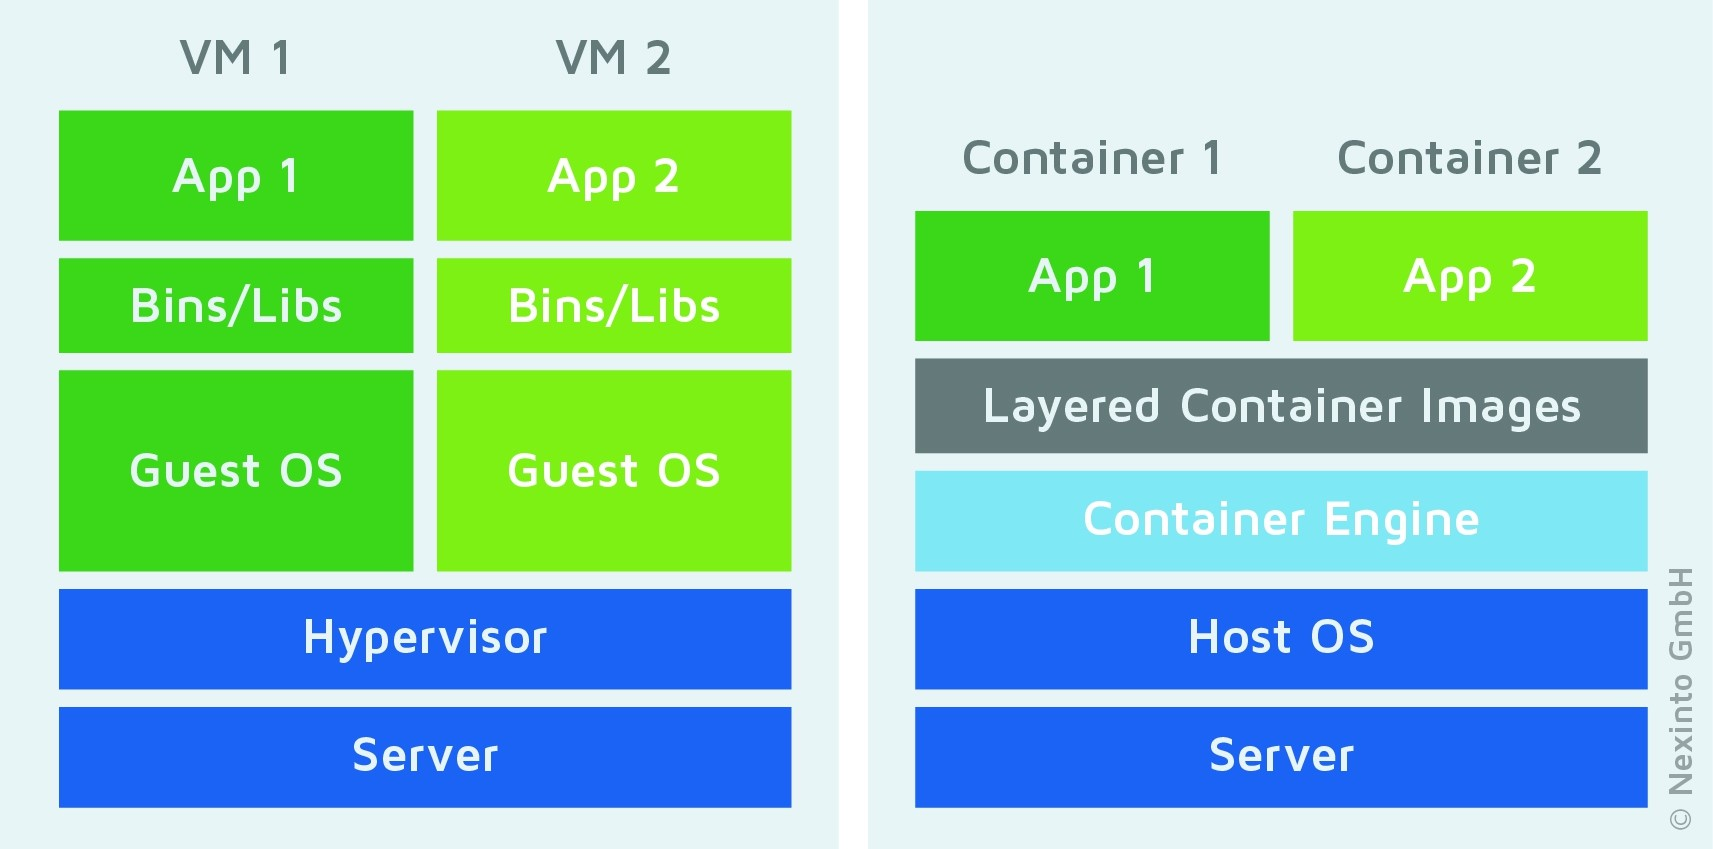
\includegraphics[width=0.7\textwidth]{containervsvm.jpg}
	\caption[Docker vs Virtual Machine Architecture]{Virtual machine architecture on the left versus container architecture on the right. Docker does not rely on a hypervisor.~\cite{Wurbs2017Docker2018.}}
	\label{container}
\end{figure}

To virtualize applications, Docker uses containers which are built up on Docker images. Images are read-only templates that are built from a set of instructions written in a Dockerfile. They offer one great advantage - a layered file system. This enables the user to easily add or update applications very quickly. Images can be shared in a public/private registry called Docker Hub. \\
Last but not least, development and operations of applications can be harmonized through a combination of Docker and a continuous integration and continuous delivery platform. 

Heroku is a platform as a service provider whose underlying technology shares some core concepts with Docker. E.g., BuildPacks are a set of scripts which are used to set up the final state of an image. The pendant on the Docker side is called Dockerfile. See Thurig's blog~\cite{Thurig2014Docker2018} for a full description of the similarities and table~\ref{dockerandheroku} for a list of pendants. However, there are also differences between the two alternatives. The main one is the dependency on the Heroku platform on the Heroku side, whereby on the Docker side one is completely flexible in choosing any environment from Raspberry Pi to cloud platform providers like Amazon Web Services. The latter also means a surplus of workload on infrastructure on the Docker side. Also, one is less flexible on the prices. Heroku has a staged price model ranging from 0 to 500\,\$ per month and dyno. Docker is again more flexible in letting one just paying for the hosting and storaging and leaving the additional features provided by Heroku aside.~\cite{Chris2017Why2018} 


\begin{table}
\begin{center}
      \caption[Similar core concepts of Docker and Heroku]{Similar core concepts of Docker and Heroku. \cite{Thurig2014Docker2018}}
  \begin{tabular}{ l | l }
    Docker & Heroku  \\ \hline
Dockerfile &	BuildPack \\ 
Image	& Slug\\ 
Container&	Dyno\\ 
Index	&Add-Ons\\ 
CLI	&CLI
  \end{tabular}
  \label{dockerandheroku}
\end{center}
\end{table}

\section{OPC UA Vision}
If two humans want to communicate with one another, they need matching channels and need to speak the same language. A channel is a mean of transport for information, e.g., sign language, smoke signs, mobile phones, etc. If one entity tries to call someone via phone if the other does not have a phone or the caller enters the wrong number and the other has its cellphone turned off, they cannot communicate. In case they both have a phone, the called entity answers and both speak a common language (e.g., English), the exchange of information can be achieved. Communication within technical systems faces the same challenges. As for the right channel, models like the \textit{Open Systems Interconnection} (OSI) basic reference model for information technology standardized by the \textit{International Organization for Standardization} (ISO) layer the transfer of information from the physical layer consisting of peaks in currents and voltages up until the application layer which includes direct user interaction, resource availability and so forth.~\cite{InternationalOrganizationForStandardization1996ISO/IECEd.} This model and the protocols adhering to it ensure that information is delivered safely between communicating entities. However, this model does not imply the semantics of the payload or the language, as stated in the analogy above. A currently proposed semantic standard for OD processes is \textbf{OPC UA Vision}. It includes a finite state machine abstracting an industrial system from its diverse conditions and transitions. Moreover, it offers an information model covering the administration of recipes, configurations and results. With the help of the state machine, it is defined which information of the information model is retrievable. The content of the three administration objects remains proprietary with the advantage of covering a broad range of OD scenarios.

\subsection{State Machine}
According to the specification, powering up and shutting down a vision system are mandatory processes and thus should be handled in a standardized manner. Also, the handling of errors should be the same for all vision systems. The design of the core operation state, however, shall remain with the manufacturer. Automatic mode as a sub-state of operational mode as is one proposed way of designing it. The state machine for a typical vision system in automatic mode is depicted in figure~\ref{fig:OPCStateMachineAutomatic}. An example of this operation would be a PLC guiding an inspection system for position determination. When powered on, the system enters the preoperational state through loading a configuration marked as active. From there, an operation mode is either automatically chosen by the system or manually triggered. An operation mode is any sub-state machine of the operational state. The automatic mode is chosen and enters the initial state. Then a recipe can be prepared, describing properties, procedures and parameters for a machine vision job. The recipe may include information for a single and/or continuous execution. A single execution would be e.g. determining the pose of an object; a continuous execution could be monitoring and surveillance systems which constantly process and acquire data. When the system is done with an execution or execution step, e.g., taking a picture from one of four angles, it sends results asynchronously to the client. If the system is shut down, it should be put into halt mode first where a safe power-off is assured. From all states, it is possible to enter the error state. Errors are handled aligning with their severity and sometimes need acknowledgment or confirm by a human before the system can be reset to preoperational state.

\begin{figure}[ht]
    \centering
    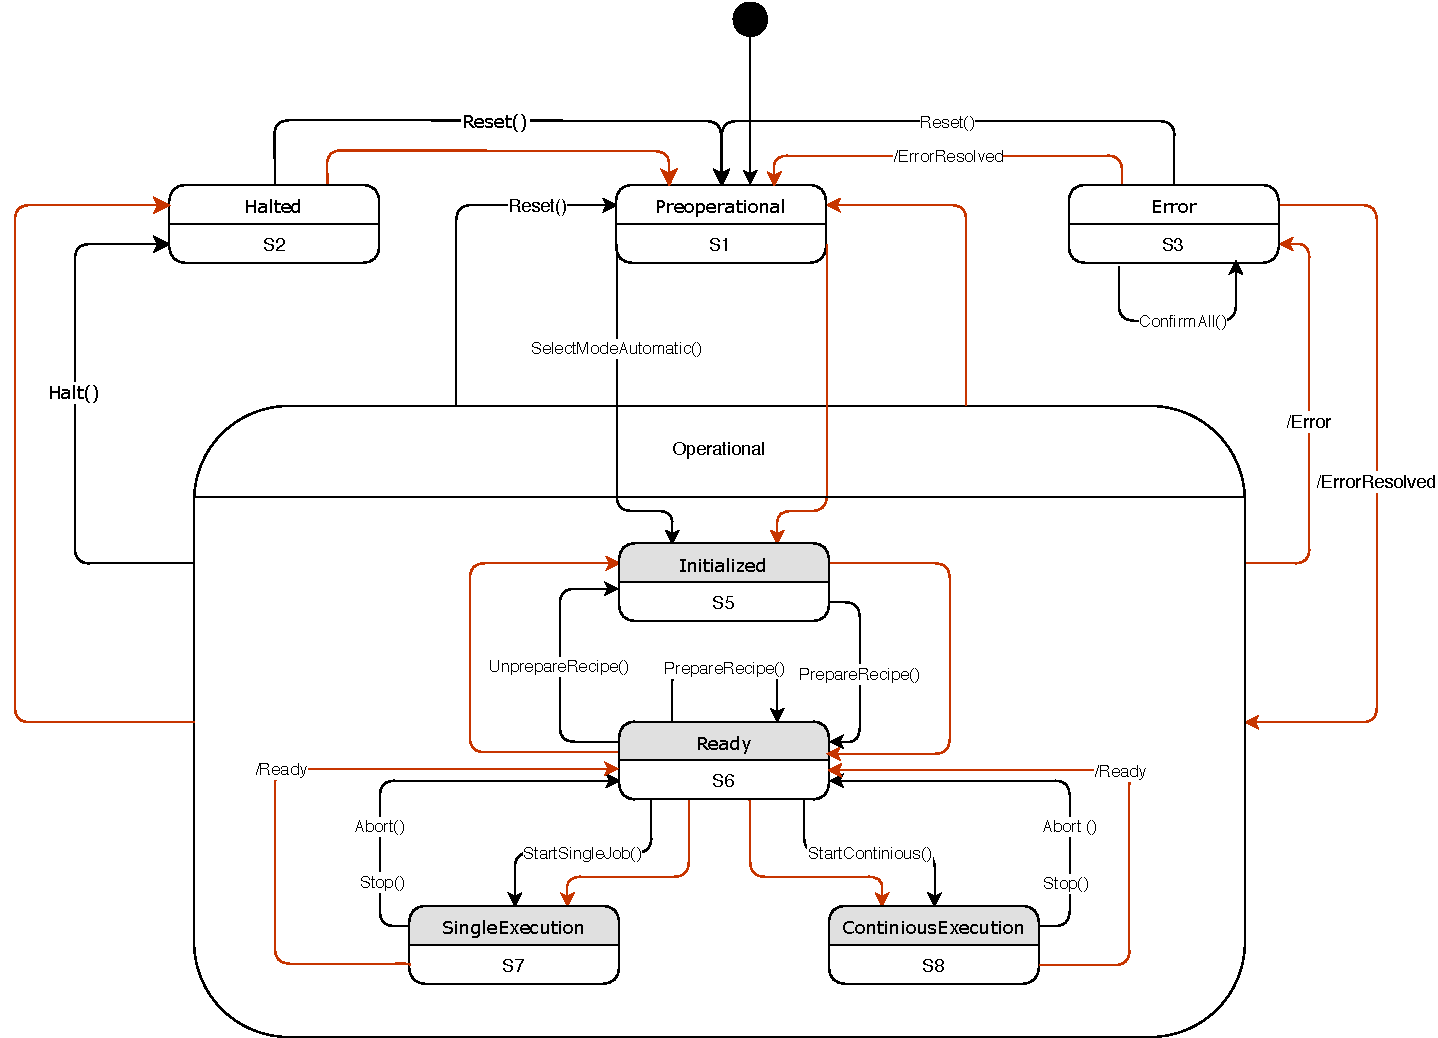
\includegraphics[width=\textwidth]{img/OPCUAVisionVisionAutomaticModeStateMachineStates.pdf}
    \caption[OPC UA Vision state machine in automatic operation mode]{OPC UA Vision state machine in automatic operation mode. Red Lines indicate automatic transitions induced by the vision system with optional effects prefixed with a slash. Black lines indicate method induced transitions with the method name as the trigger. The black circle is the entry point of the state machine. All of the states can have optional sub-state machines. States marked in grey are substates.~\cite{VDMA2018OPCSpecification}}
    \label{fig:OPCStateMachineAutomatic}
\end{figure}

\subsection{Information Model}
The information model formally describes all datasets, types, methods, address- and namespaces. See figure~\ref{fig:OPCInfoModelOverview} for an overview and figure~\ref{fig:OPCInfoModelNotation} for an explanation of the notation. 

\begin{figure}
    \centering
    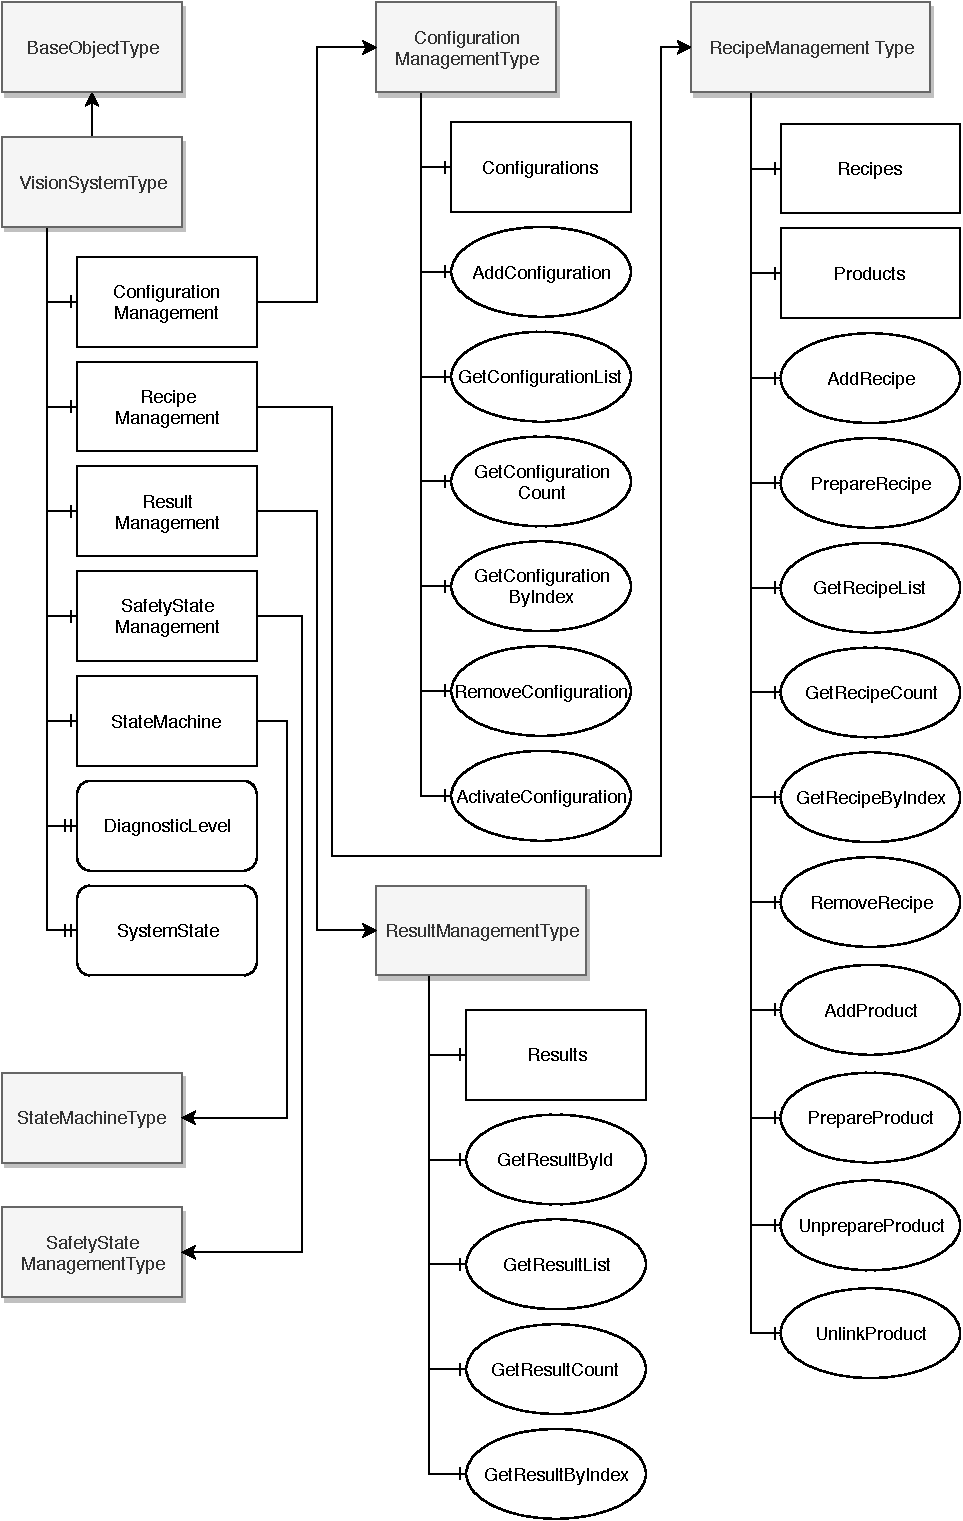
\includegraphics[height=0.9\textheight]{img/OPCUAVisionInformationModelOverview.pdf}
    \caption[OPC UA Vision Information Model Overview]{OPC UA Vision Information Model Overview. See fig. \ref{fig:OPCInfoModelNotation} for a description of the notation.~\cite{VDMA2018OPCSpecification}}
    \label{fig:OPCInfoModelOverview}
\end{figure}

\begin{figure}[ht]
    \centering
    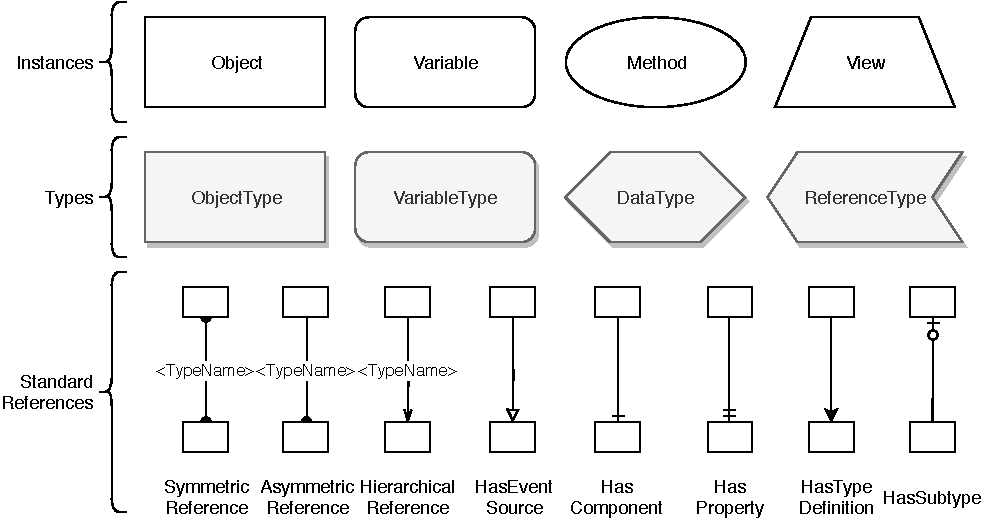
\includegraphics[width=0.8\textwidth]{img/OPCUAVisionInformationModelNotation.pdf}
    \caption[OPC UA Vision Information Model Notation]{OPC UA Vision Information Model Notation.\cite{VDMA2018OPCSpecification}}
    \label{fig:OPCInfoModelNotation}
\end{figure}

The StartSingleJob method (subpart of StateMachineType, not depicted in the overview) for example, triggers transition from state Ready to SingleExecution in~\ref{fig:OPCStateMachineAutomatic}. Its signature consists of following parameters:

\begin{tabbing}
    space \= space \= spacespacespace \= spacespacespacespace \= spacespacespace \kill
    \>  StartSingleJob(\\
    \>  \>  (in)	 \> 	String          \> MeasId\\
    \>  \>  (in)	 \> 	String          \> PartId\\
    \>  \>  (in)	 \> 	RecipeIdType    \> RecipeId\\
    \>  \>  (in)	 \> 	ProductIdType   \> ProductId\\
    \>  \>  (out)	 \> 	String          \> JobId\\
    \>  \>  (out)	 \> 	Int32           \> Error); 
\end{tabbing}

In another section of the specification, the data types are defined, e.g. RecipeIdType, which is a structure including an Id, a version and a hash.



